%! Author = hmaier
%! Date = 09.09.21

% Preamble
\documentclass[12pt,german,ngerman]{report}
\title{Künstliche Intelligenz - Ein Blick in die Zukunft?}
\author{Hendrik Maier}
\date{}


% Packages
\usepackage[T1]{fontenc} % für die spezielle Quotierung, die mit
\usepackage{german}
\usepackage{titling}
\usepackage{titlesec}
\usepackage{graphicx}
\graphicspath{ {./pictures/} }
% zeilenabstand
\usepackage[onehalfspacing]{setspace}


% quotation-marks
\usepackage[
    left = \flqq{},% the special quote on the left (opening)
    right = \frqq{},% the special quote on the right (closing)
            ]{dirtytalk} % quoting
\usepackage{csquotes}

% bibliography
%\usepackage[backend=biber,autocite=footnote,style=authortitle-ibid,babel=other]{biblatex}
\usepackage[
    backend=biber,
   % cite=footnote,
    style=numeric,
]{biblatex}
\addbibresource{ai-references.bib}

% less blank space infornt of chapters
\titleformat{\chapter}[display]
{\normalfont\huge\bfseries}{\chaptertitlename\ \thechapter}{20pt}{\Huge}

% this alters "before" spacing (the second length argument) to 0
\titlespacing*{\chapter}{0pt}{0pt}{5pt}


% Document
\begin{document}

    \begin{titlepage}
        \centering
        {\scshape\LARGE Leibniz Institut für Pflanzenbiochemie\par}
        \vspace{1cm}
        \begin{figure}[h]
            
\includegraphics[width=1.5cm]{ipb_logo.png}
            \centering
        \end{figure}
        {\huge\bfseries Künstliche Intelligenz - Ein Blick in die Zukunft?\par}
        \vspace{1cm}
        \begin{figure}[h]
            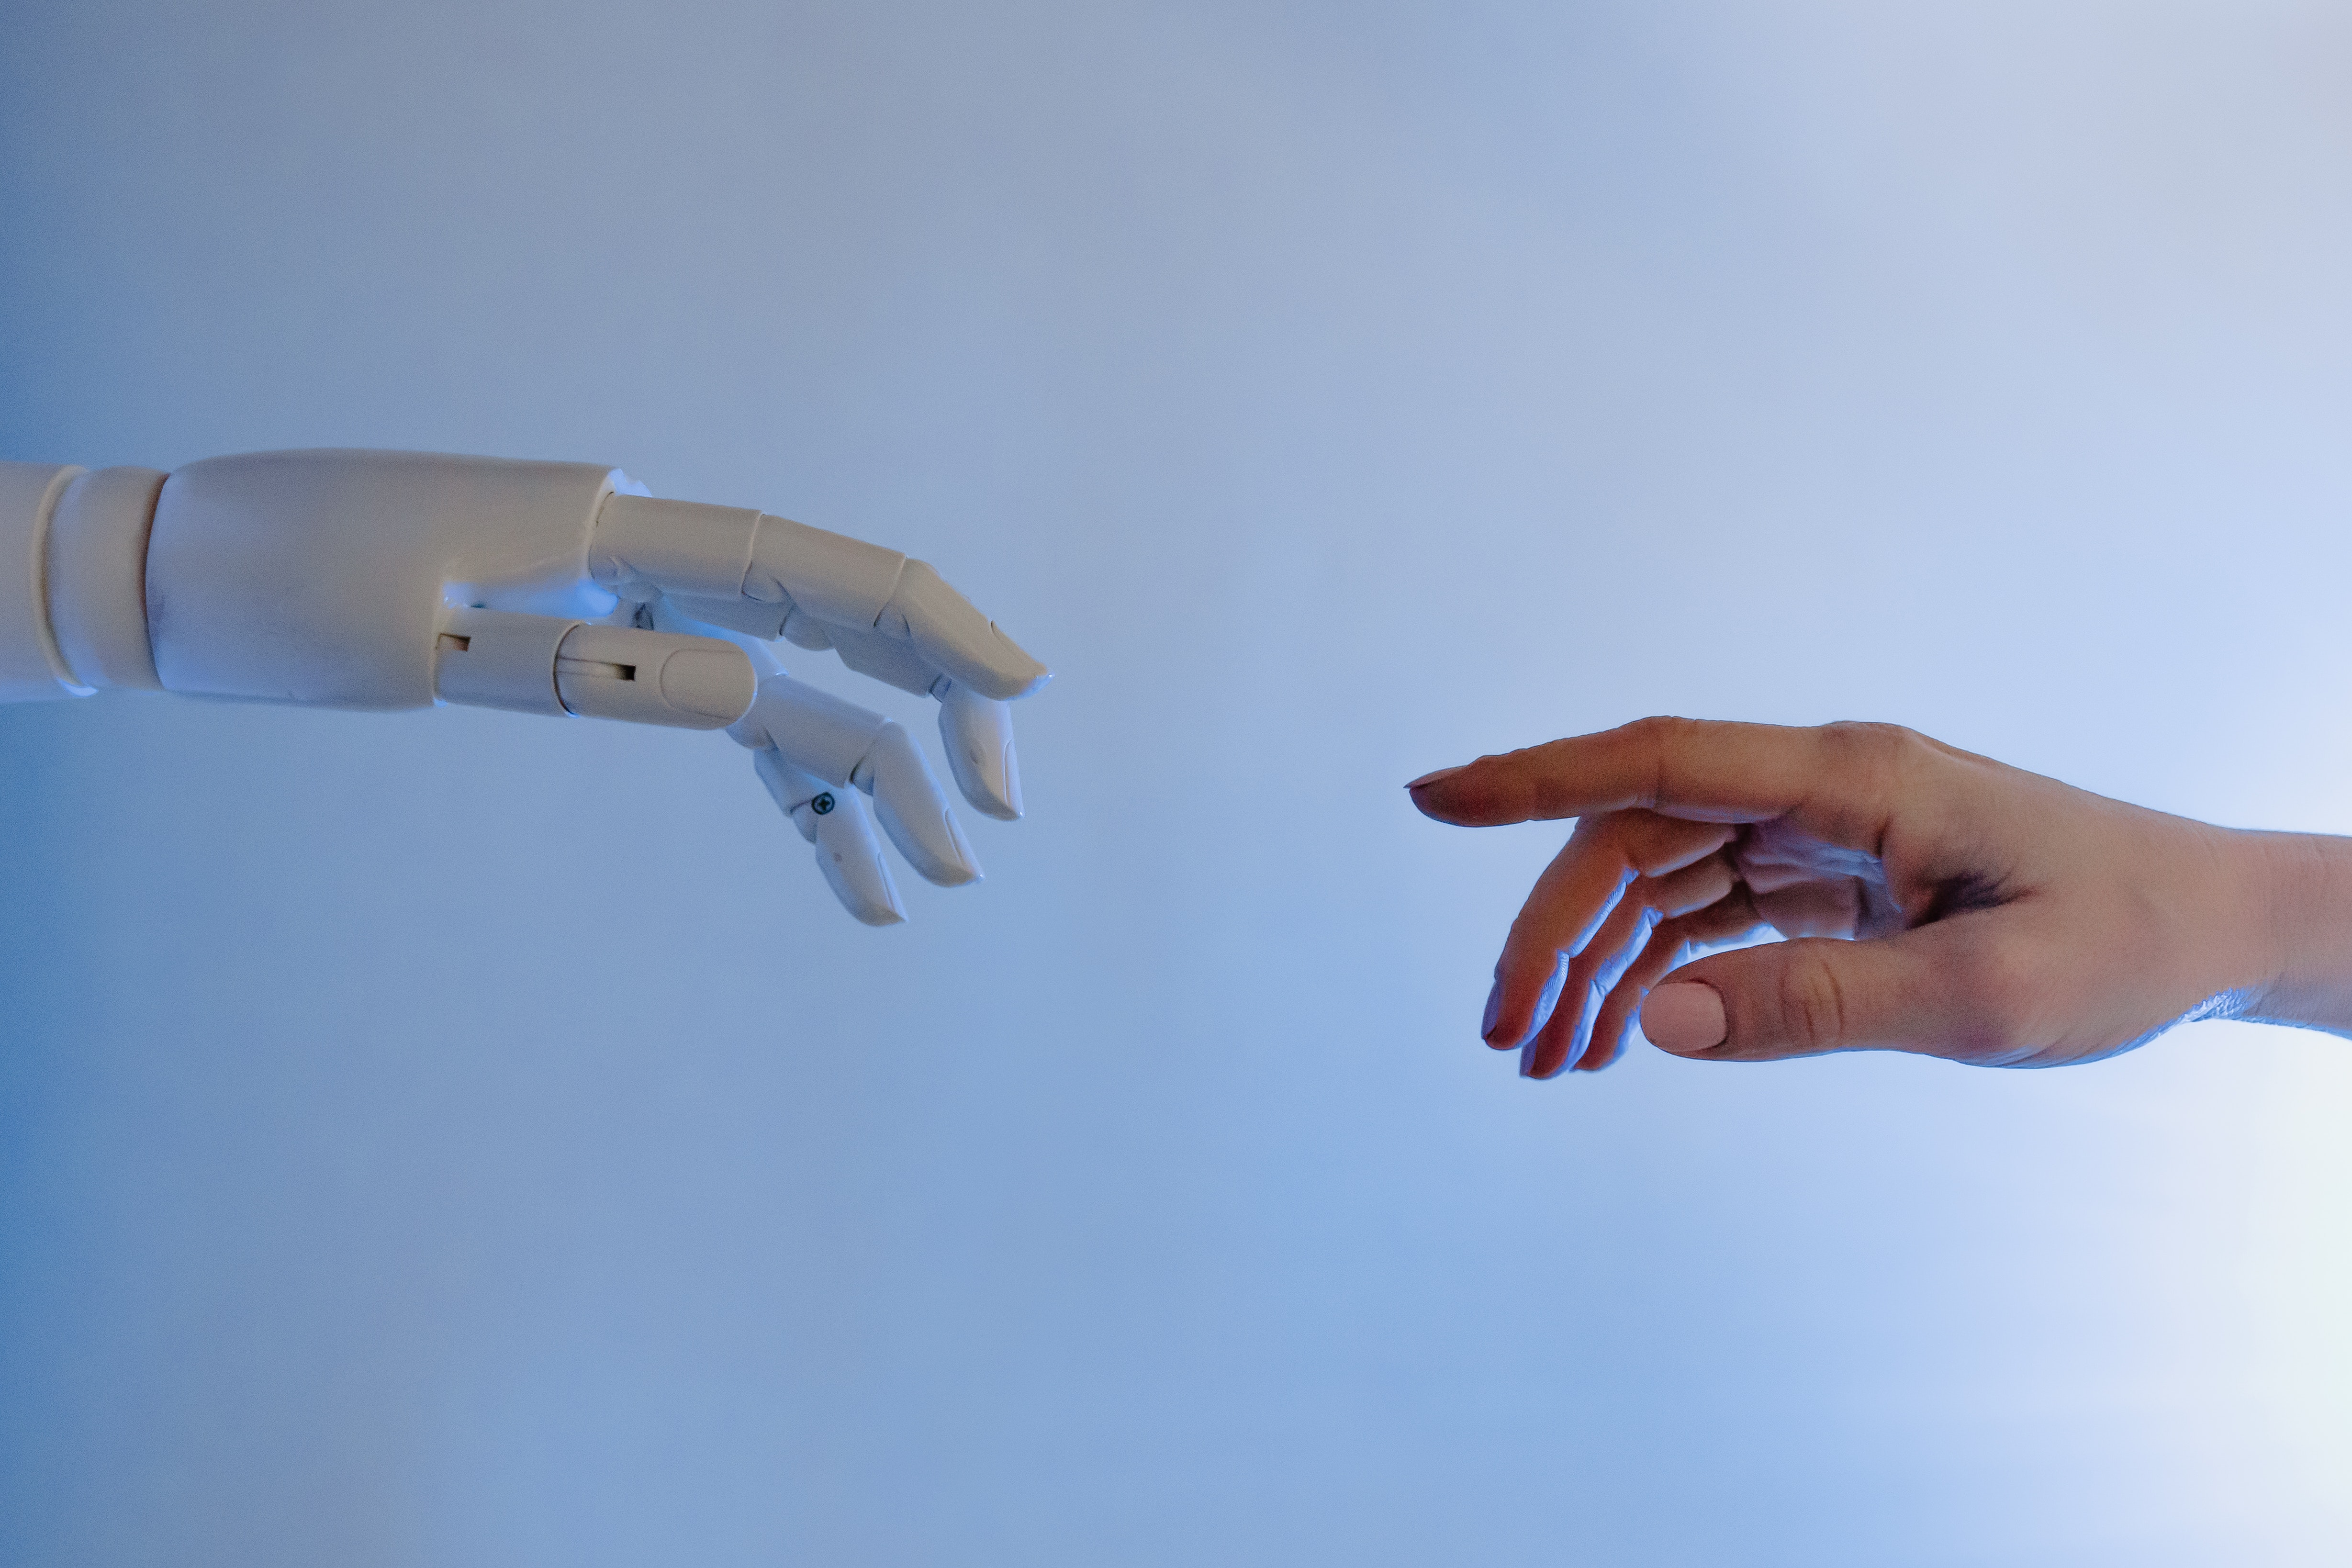
\includegraphics[width=10cm]{michelangelo_ki.jpg}
            \centering
        \end{figure}
        \vspace{1cm}
        {\Large Auszubildender Fachinformatiker Systemintegration \textbf{Hendrik Maier}\par}
        \vfill

% Bottom of the page
        % {\large \today\par}
    \end{titlepage}

    \tableofcontents
    \newpage

% Begin of the Text
\chapter{Was ist eigentlich künstliche Intelligenz - Definition und Einleitung}
    

\chapter{Der Traum vom mechanischen Helferlein - Geschichte}

Wie auch bei vielen anderen neuzeitlichen Erfindungen, spielte Kultur in Form von Literatur eine entscheidende Rollen
in der KI-Forschung. Erst durch die Vorstellungskraft von Autoren wie Isaac Asimov\footnote{bekannt durch: Die Foundation-Trilogie, derZweihunderjährige Mann}
oder Jule Verne\footnote{bekannt durch: Zwanzig Tausend Meilen unter dem Meer, Die Reise zum Mittelpunkt der Erde}, wurde Generationen
von Forschenden inspiriert die Grenzen des Möglichen auszutesten. Die Idee der KI ist dabei schon so alt wie unsere
Zivilisation. Schon der griechische Dichter Homer schrieb von mechanischen Dienern die den Göttern bei ihrem Mahl
Wein nachschenkten.\cite[53]{buchanan2005very} Auch wenn diese Verwendung eines Robotors aus unserer heutigen
industriellen Sicht eher banal erscheint, war ein solcher Apparat zu damaligen Zeiten visionär.
Nicht weniger visionär, war die Vorstellung des Philosophen und Naturforschers Gottfried Wilhelm Leibniz der mechanische
Richter imaginierte, die aufgrund von logischen Regeln Rechtsfälle zwischen Parteien aushandeln.\cite[53]{buchanan2005very}
Vergleicht man diese Vorstellungen mit der heutigen Zeit, sieht man das sich die Wünsche der Menschen durch die Zeit hindurch
nicht groß verändert haben. Leibniz und Homer beschreiben beide dienende und logisch operiende Maschinen.
Doch gestehen beide ihren erdachten Apparaten ein wesentliches Attribut nicht ein: die Denkfähigkeit. 
\section{Denkfähige Maschinen}
Um dies zu wagen braucht es Mitte des 20. Jahrhunderts erst den britischen Mathematiker Alan Turing, 
der mit seinem Gedankenexperiement, dem \say{Nachnahmungs-Spiel}, die Frage nach intelligenten und denkenden Maschinen stellte.
Dieses auch als \say{Turing-Test} bekannte, Gedankenexperiement stellt seit dem einen Richtwert für den Forschritt der KI-Forschung.\footnote{Mehr dazu im Kapitel 5, Gedankenexperimente}
Diese entstand zur gleichen Zeit als Ergebnis der Verbesserung der Halbleiter-Technologie, die als Basis für 
moderne binäre Computersysteme gilt. Die dadurch vergrößerte Rechenkapazität und -leistung eröffnete bisher nicht realisierbare Forschungsmöglichkeiten. 
Seit dem finden KI-Forschende immer mehr Anwendungsmöglichkeiten um die Grenzen der KI immer weiter auszuweiten.\\

1997 erzeugt das Schreiben und Test von KI-Programmen, erstmals einen großes Medienecho, als der von IBM programmierte Schachcomputer
\say{Deep Blue} den damals amtierenden Schach-Weltmeister Gary Kasparov, schlug.\cite{chessbase2017kasparovdeepblue} Die Komplexität von Schach war mit purer brutaler
Rechnenleistung bisher noch nicht geknackt wurden. Dazu bedarf es erst einem \say{Verständnis} von Schach dass bis zu diesem
Zeitpunkt nur Menschen zugänglich war. Das Programm probierte also nicht mehr nur alle Züge aus, sondern prognostizierte die 
Sinnvollsten. Damit wurde eine Zeitenwende eingeleitet und der breiten Öffentlichkeit die Macht von KI demonstriert.
Das dadurch erschaffene Interesse beflügelte die KI-Forschung und weitete diese in mehr Anwendungsbereiche aus.
In 2021 hatten ein Großteil der Menschen in ihrem Alltag schonmal Kontakt zu KI-Technologie. 
Ob bei der Suche im Internet oder bei Nutzung einer Sprachsteuerung, steht im Hintergrund immer diese Technologie.
Die Vorstellung von einem mechanischen Helferlein weicht allmälich dem Bild der allwissenden künstlichen Intelligenz.
\section{Zukunftsprognosen}
Eine der bekanntesten Hypothesen wurde 1993 vom US-Amerikanischen Mathematiker und Informatiker Vernor Vinge aufgestellt und 2003
erneut bestätigt. Vinge bespreibt ein spätestens 2030 auftretendes Ereignis, 
welches er die \say{technologische Singularität}\cite[1]{vinge1993technological} nennt. 
Er nennt mehrere Szenarien welche direkt oder indirekt, ein Entstehen einer denkfähigen superintelligente Entität beschreiben, 
die auf Computertechnologie basiert.\\

Betrachtet man Vinges Prognose für die nahe Zukunft\footnote{oder allein schon den heutigen Stand der Technologie mit Siri, Google und Co.} und 
Homers Beschreibung von Wein ausschenkenden Dienern,
wird ein Entwicklungsprozess sichtbar, dem jeglicher Vergleich fehlt. 



\chapter{Schwache versus Starke - Arten von KI}
     
    \section{Schwache KI}
        \subsection{}
    \section{Starke KI}
        \subsection{Technolgische Singularität}
        \subsection{künstliche Ethik}

\chapter{Technische Grundlagen}
     Wie schon zuvor beschrieben ist eine KI nichts anderes als ein Computerprogramm,
     welches durch die Analyse von Statistiken oder Datenpunkten, Prognosen abgeben oder Muster erkennen kann.
     Diesen Prozess der Analyse nennt man maschinelles Lernen (ML).
     In diesem Prozess spielen das Feld der Erkenntnistheorie, Mathematik und Informatik 
     maßgebende Rollen. Jede Disziplin erfüllt dabei eine eigene Aufgabe.
     Um eine Analyse durchzuführen benötigt es eine methodischen Ansatz.
     Die Erkenntnistheorie stellt hierfür die Methoden zur Verfügung.\footnote{Diese werden auch von 
     Menschen bewusst oder unbewusst beim Lernen und Verstehen verwendet.}
     Die Mathematik gibt die Möglichkeit diese Methoden in eine allgemeine anwendbare Sprache zu übersetzen.
     Die praktische Anwendung geschieht durch die Informatik in Form von Programmierung.
     Durch die Zusammenarbeit von diesen verschiedenen Disziplinen ist ML möglich.
        
    \section{Wie betreibt man maschinelles Lernen?}
        Im Vorfeld des Lernes, ist es wichtig den Sinn der KI zu bestimmen.
        Den je nach Anwendungsfeld oder Ziel der KI, kommt eine andere Methode und somit
        ein anderer Algorithmus zum Einsatz. Jede Methode biete verschiedene Algorithmen
        an, die jeweils eigene Vorgehen verlangen. Unter den Algorithmen kann man
        dann den passenden auswählen, der die Zielvorgabe erfüllt.

    \subsection{Top-Down Methode (Deduktiv)}
        Die erste Methode die beim ML angewandt wird, bezeichnet man als Top-Down Methode,
        welche deduktiver Natur ist. Dies bedeutet das man mithilfe von allgemein anerkannten Regeln
        auf spezielle Fälle schließt.\cite{dundi2021unileipzig} 
        Beispielweise weiß ich dass die Sonne warm ist. Da draußen die Sonne scheint, schließe ich daraus
        das es draußen warm sein muss.\footnote{Das bedeutet aber nicht das Deduktion der sicherste Weg des 
        Schlussfolgern ist. Draußen kann die Sonne scheinen und es kann kalt sein weil Winter ist.}
        Im Kontext des ML bedeutet das dass immer vorgefertigte Regeln vorhanden sein müssen.
        Diese Regeln müssen vom Menschen definiert werden. Daher spricht man bei dieser Methode
        auf vom beaufsichtigten Lernen bzw. Supervised Learning.
        \subsubsection{Supervised Learning}
            Beim Supervised Learning 
           
%        \subsection{Pre-Labeled (Test-und Training-) Data}
%        \subsection{Specific Application Area}
%        \subsection{Pro \& Contra}
        
    \subsection{Bottom-Up (Induktiv)}
        Die zweite Methode die beim ML angewandt wird, betrachtet Daten ohne davor irgendeine Form von Regeln zu beachten.  
        Die Daten werden unvoreingenommen und ohne jede Grundlage betrachtet.
        Aufgrund von logischen Zusammenhängen werden dann Regeln abgeleitet womit sich die Daten erklären lassen können.
        Diese Methoden wird, bildgebend, als Bottom-Up oder auch als induktiv\cite{dundi2021unileipzig} bezeichnet.
        \subsubsection{Unsupervised Learning}
            Die Anwendung der Bottom-Up-Methode wird im informatischen Kontext als \say{Unsupervised Learning (UL)}, oder auf deutsch als unbeausichtigtes Lernen, bezeichnet.
             
%        \subsection{Unlabeled Training Data (no Test, no Accuary)}
%        \subsection{Wide Range of Output}
%        \subsection{Pro \& Contra}
            
%    \section{deep learning - neuronale netzwerke}
%        \subsection{kann induktiv oder deduktiv arbeiten!}
%        \subsection{wie funktionieren neuronale netzwerke?}
%        \subsection{implementierung eines menschlichen gehirn mithilfe von unsupervised learning}

\chapter{Gedankenexperimente}
    Um neue Forschungsgebiete zu erschließen, ohne dabei handfest Ansätze zu haben,
    bieten sich Gedankenexperimente als nützliche Hilfsmittel an.
    Mit deren Hilfe lassen sich unreale Situationen konstruieren, durch welche man logische Schlussfolgerungen ziehen kann.
    Im folgenden werden zwei Gedankenexperimente beschrieben, die trotz ihres zunehmenden Alters, in der KI-Forschung
    immer noch Relevanz besitzen. Beide zeichnen sich dadurch aus, dass sie dem Denkenden die Möglichkeit geben sich in die
    Rolle einer Maschine zu versetzten. Dadurch kann der Denkende die Kernfrage der KI-Forschung aus einer anderen
    bzw. aus einer eigenen Perspektive erleben. 

    \section{The Imitation Game - Das Nachahmungs-Spiel}
        Mitte des 20. Jahrhunderts stellte der britische Mathematiker Alan Turing als einer der ersten
        die Frage ob es möglich sei dass Maschinen denken könnten. Dies gilt seit dem als hauptsächliche
        Kernfrage der KI-Forschung. Um diese Frage zu beantworten schlägt Turing das \say{Imitation Game} oder
        auch \say{Nachahmungs-Spiel}, als Test für die Denkfähigkeit von Maschinen vor. Als Maschine schlägt er
        explizit einen digitalen oder elektronischen Computer vor und schließt biologische Möglichkeiten,
        wie einen aus einer Zelle gezüchteten Menschen komplett aus.\cite[435]{turing1950computing}
        Eine vollständige Abkapselung einer digitalen Maschine, als eigenständiges Gerät ist jedoch nicht möglich, das sie auf dem
        Fundament von menschlichen Prinzipien konstruiert worden ist. Maschinen müssen immer als menschgemacht gedacht werden.
        Mit diesem Hintergrundwissen schlägt er folgendes Spiel vor:
        \begin{displayquote}
            Für das Nachahmungs-Spiel werden insgesamt drei Spieler*innen benötigt. Ein Mann (A), eine Frau (B) und ein*e
            Fragesteller*in (C). Die Aufgabe des/der Fragesteller*in ist herrauszufinden wer von beiden die Frau ist.
            Dabei sitzt er/sie in einem anderen Raum als die beiden. Der/Die Fragesteller*in kennt beide Parteien
            nur unter X und Y, womit er am Ende des Spiel jeweils A und B identifiziert. Ziel von A ist es den/die Fragesteller*in
            fehlzuleiten. B verfolgt das Ziel, den/die Fragesteller*in zur richtigen Antwort zu leiten.
            \cite[433]{turing1950computing}
        \end{displayquote}
        In diesem Gedankenexperiement wird der Mann (A) nun durch eine Maschine ersetzt, die seine Aufgabe übernimmt und
        sich als Frau (B) ausgeben soll. Der Austausch von Informationen erfolgt dabei über Maschinenschrift, damit
        der/die Fragesteller*in keine Schlussfolgerungen über Stimme oder Schrift ziehen kann.\cite[433]{turing1950computing}
        Bei diesem Test geht es nicht darum akutelle Maschinen zu betrachten und ein entgültigen Schluss zu ziehen. Es geht
        eher darum sich eine Maschine vorzustellen die diesen Test bestehen kann. Damit eine Maschine diesen Test besteht
        muss sie das Spiel mit einer 70\%iger Genauigkeit gewinnen.\cite[1]{oppy&dowe2020turingtest}
        

    \section{Das Chinesische Zimmer}
    Das Chinesische Zimmer ist ein Gedankenexperiment vom Philosophen John Searle welches
    versucht die Frage nach der erfolgreiche Entwicklung einer starken Künstlichen Intelligenz zu verneinen.
    Searles These ist, dass kein Computer jemals wie ein Menschen denken kann,
    obwohl sowohl der Computer als auch das Gehirn beides Systeme sind Symbole verarbeiten.\cite{nimtz2013chinesische}
    Dies begründet er mit folgendem Gedankenexperiment:
    \begin{displayquote}
        Stellt euch vor ich wäre in einem geschlossenen Raum mit einem großen Haufen chinesischer Texte.
        Ich kann weder Chinesisch sprechen noch lesen oder schreiben.
        Ebenfalls könnte ich chinesische von keiner anderen, wie beispielweise russischer, japanischer Schrift unterscheiden.
        Chinesische Schriftzeichen haben keine erkennbare Bedeutung und sind nur Formen für mich.\\

        Nun stellt euch vor ich würde einen zweiten Stapel erhalten. Dieser Stapel enthält weitere
        Chinesische Schriftzeichen sowie englische formale Regeln, die ich ohne Probleme verstehe.
        Diese formalen Regeln geben mir die Möglichkeit die chinesischen Schriftzeichen
        anhand ihrer Form zu identifizieren.\\

        Nun kriege ich einen dritten Stapel mit weiteren chinesischen Schriftzeichen und englisch Anweisungen die mir sagen wie ich
        diese neuen chinesischen Zeichen mit den Vorherigen vergleiche um bestimmte chinesische Zeichen zurückzugeben.\\

        Mit der Zeit werden die Leute außerhalb des Raumes immer besser mir Englische Anweisungen zu schreiben und
        ich werde immer besser diese auch zu verstehen, so dass meine Antworten ununterscheidbar von denen eines
        gebürtigen Chinesen werden. Doch verstehe ich, was ich an Chinesisch von mir gebe?
        \cite[1]{searle1999chinese}
    \end{displayquote}
    Searle versucht mit diesem Gedankenexperiment den Unterschied zwischen
    Syntaktik\footnote{Syntaktik (Syntax): Wie stellt man Zeichenketten zusammen, so dass sie Sinn ergeben?}
    und Semantik\footnote{Semantik: Was genau ist die Bedeutung hinter einem Wort?}
    greifbar zu machen.
    Ein Computer der keinerlei Verbindung in die Realität eines Menschen hat, kann zwar Regel lernen, die ihm die
    Welt der Menschen näher bringt, jedoch kann er niemals voll und ganz \emph{verstehen} oder auch \emph{begreifen},
    wie ein Mensch denkt. Damit setzt Searle eine eher negative Prognose auf den Forschritt, den die KI-Forschung
    machen wird oder besser gesagt, nicht machen wird.


\chapter{Schlussfolgerung}
    \section{Unterschied Mensch und Maschine}
        Im vorherigen wurde der Begriff, die Arten sowie die Technologie an sich beschrieben und erläutert.
        Doch um wahrhaftiges Verständnis von künstlicher Intelligenz zu gewinnen, braucht es einen
        Vergleich der viel näher an dem eigenen Verständnis von Intelligenz liegt.
        Die Rede ist vom direkten Vergleich mit dem Menschen.

    \section{Menschen lernen sich selbst besser kennen wenn sie KI erforschen}
            
    \section{Was Maschinen vom Menschen unterscheidet}


    \printbibliography[title={Quellenverzeichnis}]
\end{document}
